\chapter{Positive Density from the Backward Tree}\label{chap:backward}

The density theorems of \cref{chap:divergence} fall short in two different ways. The bound of Krasikov and Lagarias (\cref{sec:ch9:krasikov}) counts integers that provably reach $1$, but only about $x^{0.84}$ of those up to $x$, a proportion that tends to zero. Tao's theorem (\cref{sec:ch9:tao}) covers almost every integer, but in logarithmic density and only down to a bound $f(n)$ that must tend to infinity, so it gives no proportion of integers that reach $1$. In September and October 2026 four preprints closed the first of these gaps. Mazur\index{Mazur, L.} proved that for every $t$ not divisible by $3$ the integers whose orbit passes through $t$ have positive lower density, and that a positive proportion of integers reach $1$ within $10.46\log n$ steps of $T_0$~\cite{mazur2026pred,mazur2026time}. Shaik\index{Shaik, I. A.} lowered the constant to any $c>3/\log(4/3)\approx10.428$~\cite{shaik2026}. Lau\index{Lau, K.} gave a quantitative refinement, with a much smaller tower of constants, explicit dependence on the target and step bounds for every target $t$ not divisible by $3$, in a preprint whose mathematics and Lean formalization were produced by the AxiomProver\index{AxiomProver} system~\cite{lau2026}.

This chapter describes what these results say, how the proof is built and what they change for the conjecture, and it tests their numerical side. The proof runs the dynamics backwards: it counts the predecessors of a target in the inverse tree\index{inverse tree}, weighs each by a power of $3$ over a power of $2$, and needs only that residues modulo powers of $3$ mix. The rest of this book runs forwards, along orbits, and the two are dual views of the same random walk, the stride model of \cref{def:ch3:models}. The results are recent and have not been refereed. We have compared the statements quoted here with the texts of the preprints and with Lau's Lean statements, and our own computations agree with every number we report from them, but we have not checked the proofs. Where a consequence is ours rather than the preprints', we say so. \Cref{sec:ch9b:duality} makes precise in what sense the forward model is $2$ adic and the backward model is $3$ adic.

\section{The theorems}\label{sec:ch9b:theorems}

We write $\sigma_0(n)$ for the number of steps of $T_0$ that take $n$ to $1$, the total stopping time of \cref{chap:intro}, and $A(n)$ for the number of odd values among $n,T_0(n),\ldots,T_0^{(\sigma_0(n)-1)}(n)$. For odd $n$, $A(n)$ is the number of steps of the Syracuse map $S$ that take $n$ to $1$. Lau calls the steps of $T_0$ ordinary steps and those of $S$ accelerated steps; the accelerated map $T$ of this book counts neither. Logarithms are natural, and
\[
  D_A=2^{2^{2^{87640}}} .
\]

\begin{theorem}[{Lau~\cite[Theorem~1.3]{lau2026}}]\label{thm:ch9b:lau}
Let $t\ge1$ with $3\nmid t$, and let $X\ge2^{t^3D_A}$. At least $t^{-4}D_A^{-1}X$ odd integers $n<X$ reach $t$ within $10.46\log(n/t)$ steps of $T_0$ and reach the odd part of $t$ within $3.4881\log(n/t)$ steps of $S$.
\end{theorem}

For $t=1$ this is Lau's Corollary~1.2: for every $X\ge2^{D_A}$, at least $X/D_A$ odd integers $n<X$ have $\sigma_0(n)\le10.46\log n$ and $A(n)\le3.4881\log n$. So the integers that reach $1$, and do so in logarithmic time, have positive lower density\index{positive density}. The constants are towers of exponentials and the proportion they guarantee is unimaginably small; \cref{sec:ch9b:steps} shows that the true proportion meeting these step bounds is about one half at every size we can test.

Mazur proved positive density in two manuscripts dated 6 September 2026. The first~\cite[Theorem~1.1]{mazur2026pred} shows that for every $a$ with $3\nmid a$ the set of integers whose orbit under $T_0$ reaches $a$ has positive lower natural density, with a constant depending on $a$, without assuming that $a$ reaches $1$ or that it lies off a cycle. The second~\cite[Theorem~1.1]{mazur2026time} shows that at least $cX$ positive integers $n<X$ have $\sigma_0(n)\le\frac{523}{50}\log n$ once $X\ge X_0$, where $\frac{523}{50}=10.46$ and $c$ and $X_0$ are explicit, given by finite arithmetic expressions~\cite[eq.~(8.6)]{mazur2026time}; Lau's Appendix~B estimates them as $c=D_M^{-1}$ and $X_0=D_M$, with $D_M$ a tower of seven $2$s topped by $173$. Earlier, in July 2026, Mazur had proved the almost bounded theorem of Tao in natural density: for every $f$ tending to infinity, almost every $n$ in natural density has an iterate $T_0^{(k)}(n)<f(n)$ with $k\le C\log n$, for an explicit $C<436$~\cite{mazur2026natural}, as described in~\cite{mazur2026time}. Shaik~\cite{shaik2026}, building on Mazur's construction, obtains positive lower density for convergence within $c\log x$ steps of $T_0$, for the integers below $x$, for every $c>3/\log(4/3)$, with one density bound for all such $c$, and the same range of times for every target not divisible by $3$. Lau's contribution is a quantitative refinement: constants of the size of a tower of height four in place of seven, explicit dependence on the target, step bounds for a general target, which Mazur's first manuscript leaves outside its scope, and a Lean certificate. The condition $3\nmid t$ cannot be dropped: if $3\mid t$, the only predecessor of $t$ under $T_0$ is $2t$, again a multiple of $3$, so the integers whose orbit reaches $t$ are the $2^kt$, a set of density zero (\cref{ex:ch9b:three}).

Lau's preprint and Mazur's two manuscripts were written with substantial help from AI systems, and each says so. Lau's states that AxiomProver autonomously produced the mathematics of the paper and formalized it in Lean, and that the human author is accountable for the statements and conclusions of the introduction and wrote the outline of the argument in its Section~2. Mazur's state that the ProofAtlas.ai harness and OpenAI models contributed substantially to exploration, proof development, formalization and exposition, and that Mazur directed the research and is responsible for the claims; the first adds that it underwent automated reviews, not human peer review, and each comes with a Lean~4 formalization. Lau's Lean files are in a public repository, AxiomMath/CollatzPositiveDensity, written for Lean~4 with the Lean mathematical library. Its challenge file, written by humans, states Corollary~1.2, \cref{thm:ch9b:lau} and Remark~1.4 of the paper with the same constants, step bounds and counts, and we have read those statements; the repository reports that its proofs were checked against them with the Lean comparator, allowing only the standard axioms of propositional extensionality, quotient soundness and choice, and its automatic build succeeds. We have not run the check ourselves. These results join the machine checked work on the sibling problem of Erd\H{o}s~$125$ and our own Lean statements in \cref{sec:ch8:lean}.

The most important consequence for this book is a conditional statement with a three line proof. Mazur states it with upper density~\cite[Corollary~1.2]{mazur2026pred} and Lau with natural density~\cite[Corollary~1.6]{lau2026}; the proof is the same.

\begin{corollary}[{Density one suffices}]\label{cor:ch9b:densityone}
If the set of $n$ whose orbit reaches $1$ has upper natural density one, then every orbit reaches $1$.
\end{corollary}

\begin{proof}
Suppose the orbit of $t$ never reaches $1$. Some point of that orbit is prime to $3$: if $3\mid t$, halve until the value is odd and apply $T_0$ once more, which gives a value $\equiv1\pmod3$. Replace $t$ by that point. Then $t\notin\{1,2,4\}$, and by Mazur's theorem, or by \cref{thm:ch9b:lau}, the integers whose orbit reaches $t$ have positive lower density. None of them reaches $1$: an orbit that met $1$ before $t$ would stay in the cycle $1,4,2$ and never meet $t$, and an orbit that meets $t$ follows the orbit of $t$ from then on. So the integers that do not reach $1$ have positive lower density, and those that do have upper density less than one.
\end{proof}

The following consequences are ours; they are not stated in the preprints, but they follow at once.

\begin{proposition}[A bounded form of Tao's theorem would suffice]\label{prop:ch9b:bounded}
Assume the positive density theorem (\cref{thm:ch9b:lau}, or Mazur~\cite[Theorem~1.1]{mazur2026pred}) and that every integer up to $2^{71}$ reaches $1$~\cite{barina2025}. (a) If the set of $n$ whose orbit reaches $1$ has logarithmic density one, then every orbit reaches $1$. (b) If $\mathrm{Col}_{\min}(n)\le2^{71}$ for all $n$ in a set of logarithmic density one, then every orbit reaches $1$.
\end{proposition}

\begin{proof}
For every set of integers the lower natural density is at most the lower logarithmic density, which is at most the upper logarithmic density, which is at most the upper natural density (\cref{ex:ch9b:densities}). So for (a), logarithmic density one, the density of Tao's theorem, implies upper natural density one, and \cref{cor:ch9b:densityone} applies. For (b), every $n$ in the set reaches an integer at most $2^{71}$, and so reaches $1$. The set of $n$ whose orbit reaches $1$ therefore contains a set of logarithmic density one, so it has logarithmic density one, and (a) applies.
\end{proof}

\Cref{thm:ch1:tao} proves the hypothesis of (b) with $2^{71}$ replaced by any function $f(n)$ that tends to infinity; Mazur's theorem of July 2026 proves it in natural density, again with $f(n)\to\infty$. Tao expected the step from an unbounded $f$ to a bounded one to be almost as hard as the conjecture itself~\cite[Remark~1.4]{tao2022}. If the positive density theorems are right, it is exactly as hard, and the whole problem sits in the gap between a slowly growing $f$ and a constant.

This qualifies a point made twice earlier in the book, that no density statement, however strong, reaches every integer (\cref{sec:ch1:density,sec:ch9:tao}). A density statement about orbits becoming small still does not. A density statement about orbits reaching $1$ now does, through \cref{cor:ch9b:densityone}, because the predecessors of any orbit that missed $1$ would form a set of positive density.

\section{Words, weights and offsets}\label{sec:ch9b:words}

Run the Syracuse map backwards. The odd predecessors of an odd $x$ under $S$ are the integers $(2^ax-1)/3$ with $a\ge1$ and $2^ax\equiv1\pmod3$: an odd $x$ prime to $3$ has infinitely many, and a multiple of $3$ has none. \Cref{sec:ch9:krasikov} describes the same tree for $T_0$.

\begin{definition}[Backward words]\label{def:ch9b:words}
A \emph{word} is a finite sequence $w=(a_1,\ldots,a_d)$ of positive integers, of \emph{length} $|w|=d$ and \emph{degree} $\deg w=a_1+\cdots+a_d$. For odd $n$ put $x_0=n$ and $x_i=(2^{a_i}x_{i-1}-1)/3$ for $1\le i\le d$. The word is \emph{valid at $n$} if every $x_i$ is an integer, and then $\src(w,n)=x_d$ is its \emph{source}. Its \emph{weight} and \emph{offset} are
\[
  \wt(w)=3^d2^{-\deg w},\qquad \off(w)=\sum_{i=1}^{d}3^{i-1}2^{-(a_1+\cdots+a_i)} .
\]
\end{definition}

\begin{proposition}[The offset identity]\label{prop:ch9b:offset}
Let $n$ be odd and $w=(a_1,\ldots,a_d)$ a word. Then $w$ is valid at $n$ if and only if $n\equiv\off(w)\pmod{3^d}$, with $2$ inverted modulo $3^d$. If it is, the $x_i$ are positive odd integers with $\vt(3x_i+1)=a_i$ and $S(x_i)=x_{i-1}$, so that the source reaches $n$ in $d$ steps of $S$ and $d+\deg w$ steps of $T_0$, and
\begin{equation}\label{eq:ch9b:offset}
  n=\wt(w)\,\src(w,n)+\off(w) .
\end{equation}
Weights and offsets compose like the affine maps of \cref{prop:ch2:affine}: $\wt(vw)=\wt(v)\wt(w)$ and $\off(vw)=\off(v)+\wt(v)\off(w)$.
\end{proposition}

\begin{proof}
The composition rules follow from the definitions by splitting the sum for $\off(vw)$ after the letters of $v$. Solving the definition of $x_i$ for $x_{i-1}$ gives $x_{i-1}=(3x_i+1)2^{-a_i}$, and iterating this for the prefix $u=(a_1,\ldots,a_i)$ gives $n=\wt(u)x_i+\off(u)$, whether or not $x_i$ is an integer. Multiplying by $2^{\deg u}$,
\[
  3^ix_i=2^{\deg u}n-N_u,\qquad N_u=2^{\deg u}\off(u)=\sum_{j=1}^{i}3^{j-1}2^{a_{j+1}+\cdots+a_i},
\]
and $N_u$ is an integer, so $x_i$ is an integer if and only if $n\equiv\off(u)\pmod{3^i}$. Since $\off(w)-\off(u)=\wt(u)\off(a_{i+1},\ldots,a_d)$ is divisible by $3^i$ in the $3$ adic integers, the condition for $i=d$ implies it for every $i\le d$. If $x_i$ is an integer, then $2^{a_i}x_{i-1}-1$ is odd, so $x_i$ is odd; $x_i>0$ when $x_{i-1}\ge1$; and $3x_i+1=2^{a_i}x_{i-1}$ with $x_{i-1}$ odd, so $\vt(3x_i+1)=a_i$ and $S(x_i)=x_{i-1}$. The case $i=d$ is \eqref{eq:ch9b:offset}.
\end{proof}

\begin{example}[The word of $11$]\label{ex:ch9b:eleven}
The Syracuse orbit $11\to17\to13\to5\to1$ has letters $a=\vt(3n+1)$ equal to $1,2,3,4$ along the way. Read backward from the target $1$ the word is $w=(4,3,2,1)$: $x_1=(16-1)/3=5$, $x_2=(40-1)/3=13$, $x_3=(52-1)/3=17$, $x_4=(34-1)/3=11$. The word has length $4$ and degree $10$, and $11$ reaches $1$ in $4$ steps of $S$ and $14$ steps of $T_0$. Its weight and offset are $\wt(w)=81/1024$ and $\off(w)=133/1024$, and \eqref{eq:ch9b:offset} reads $1=\frac{81}{1024}\cdot11+\frac{133}{1024}$.
\end{example}

\Cref{eq:ch9b:offset} turns counting predecessors into weighing words. Since $\off(w)>0$, a word valid at $t$ has $\wt(w)<t/\src(w,t)$. Counting sources, rather than words, needs a target that is not on a cycle of $S$.

\begin{lemma}[{Distinct words, distinct sources: Lau~\cite[Lemma~3.3]{lau2026}}]\label{lem:ch9b:distinct}
Let $t$ be an odd positive integer with $S^{(r)}(t)\ne t$ for every $r\ge1$. Then distinct words valid at $t$ have distinct sources.
\end{lemma}

\begin{proof}
Let $w$ be valid at $t$ with source $s$. Read the inverse trajectory forward from $s$: the next value on the forward orbit of $x'$ is $(3x'+1)/2^{a}$, and this is an odd integer only for $a=\vt(3x'+1)$. So $s$ and the length $|w|$ determine $w$, and $S^{(|w|)}(s)=t$. If two lengths $r<r'$ both had $S^{(r)}(s)=S^{(r')}(s)=t$, then $S^{(r'-r)}(t)=t$, which was excluded. So $s$ determines $|w|$, hence $w$.
\end{proof}

So for a target $t$ off the cycles of $S$ and any family of words valid at $t$ whose sources lie in a window $[X,32X)$,
\begin{equation}\label{eq:ch9b:reduction}
  \#\{\text{sources in }[X,32X)\}\;\ge\;\frac{X}{t}\,\beta_X(t),
\end{equation}
where $\beta_X(t)$ is the total weight of the family. A lower bound on $\beta_X(t)$ that does not depend on $X$ is a positive lower density for the predecessors of $t$, and the whole proof is such a lower bound. A target on a cycle is handled through a suitable predecessor off the cycle~\cite{mazur2026pred}.

It is worth seeing what $\beta_X(t)$ is before the proof bounds it from below, and the target $t=1$ is the natural test. It lies on a cycle of $S$, since $S(1)=1$ with the letter $2$, so \cref{lem:ch9b:distinct} does not cover it as it stands: the words $(2)$, $(2,2)$ and so on are all valid at $1$ with the source $1$, and every odd source $s>1$ is the source of the words $(2,\ldots,2,w_s)$ as well as of $w_s$, the word of its Syracuse orbit down to its first visit to $1$. We count each source once, by $w_s$, and write $\beta_X(1)$ for the total weight of these words over the sources in $[X,32X)$; the sources are distinct by construction, so \eqref{eq:ch9b:reduction} holds for this family. Every integer up to $2^{71}$ reaches $1$~\cite{barina2025}, so every odd $n<2^{24}$ is a source, and for $X\le2^{19}$ the window $[X,32X)$ lies below $2^{24}$ and $\beta_X(1)$ is computed from the Syracuse orbit of every odd integer in it. \Cref{tab:ch9b:tree} gives the result, and \cref{fig:ch9b:tree} shows the first levels of the tree.

\begin{figure}[t]
\centering
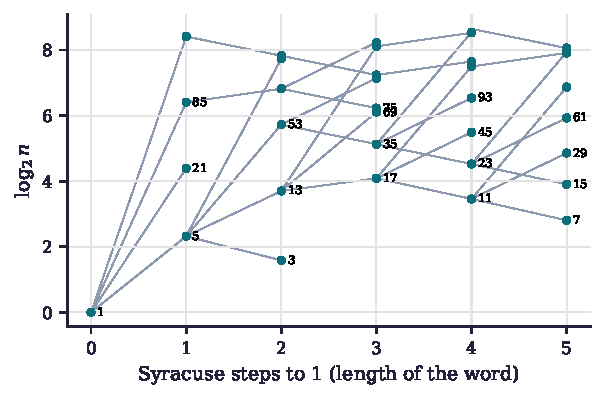
\includegraphics[width=\textwidth]{figures/ch9b_tree.pdf}
\caption{The bottom of the backward tree from $1$: the odd integers below $400$ within five steps of $S$ of $1$, by the length of their word and $\log_2n$. Each edge is one step of $S$; the self loop at $1$, where $S(1)=1$ with the letter $2$, is not drawn.}
\label{fig:ch9b:tree}
\end{figure}

\begin{table}[t]
\centering\footnotesize
\setlength{\tabcolsep}{4pt}
\caption{The backward tree from $1$ below $2^{24}$, exactly. Every odd $n<2^{24}$ reaches $1$, so every odd integer of a window is a source, and each source $s$ is counted once, by the word $w_s$ of its Syracuse orbit down to its first visit to $1$. The second column counts the odd integers in $[X,32X)$, all of them sources; the third counts the sources that a search of the tree truncated at $2^{24}$ finds, and the others have orbits that rise above $2^{24}$ before reaching $1$, so they are lost to the truncation, not to the conjecture. The last column is $31/(2\beta_X(1))$.}
\label{tab:ch9b:tree}
\begin{tabular}{@{}rcccc@{}}
\toprule
$X$ & odd in $[X,32X)$ & found & $\beta_X(1)$ & count$/(X\beta_X)$ \\
\midrule
$2^{4}$ & $248$ & $248$ & $1.5000$ & $10.33$ \\
$2^{6}$ & $992$ & $992$ & $1.4964$ & $10.36$ \\
$2^{8}$ & $3968$ & $3968$ & $1.4918$ & $10.39$ \\
$2^{10}$ & $15\,872$ & $15\,869$ & $1.4889$ & $10.41$ \\
$2^{12}$ & $63\,488$ & $63\,335$ & $1.4892$ & $10.41$ \\
$2^{14}$ & $253\,952$ & $250\,757$ & $1.4897$ & $10.41$ \\
$2^{16}$ & $1\,015\,808$ & $962\,404$ & $1.4892$ & $10.41$ \\
$2^{18}$ & $4\,063\,232$ & $3\,189\,369$ & $1.4891$ & $10.41$ \\
$2^{19}$ & $8\,126\,464$ & $4\,720\,635$ & $1.4891$ & $10.41$ \\
\bottomrule
\end{tabular}
\end{table}

Three things are visible in \cref{tab:ch9b:tree}. First, the total weight is nearly the same in every window, but not exactly: $\beta_X(1)$ falls from $1.5000$ at $X=2^4$ to $1.4889$ at $2^{10}$, and then stays between $1.4889$ and $1.4897$ up to $2^{19}$. The harmonic sum does not explain the value: over the odd $s$ in a window of ratio $32$, $\sum1/s=\frac12\log32+O(X^{-2})\approx1.733$, not $1.49$. For the target $1$, \eqref{eq:ch9b:offset} gives $\wt(w_s)\,s=1-\off(w_s)<1$ for every source, and by \cref{prop:ch9b:steps} this is $3^{A(s)}s/2^{H(s)}=2^{-\varepsilon(s)}$, so that
\[
  \beta_X(1)=\sum_{s}\frac{2^{-\varepsilon(s)}}{s},
\]
the sum over the odd $s$ in $[X,32X)$. The mean of $2^{-\varepsilon(s)}$ over the window, weighted by $1/s$, is $\beta_X(1)/\bigl(\frac12\log32\bigr)$, between $0.859$ and $0.866$ in every row. It is set mostly by the last few odd values of the orbit before $1$, where $1/(3m_i)$ is not small, and its stability from window to window is the empirical fact that the table shows. Second, the reduction \eqref{eq:ch9b:reduction} loses the factor in the last column, $31/(2\beta_X(1))\approx10.41$. It splits as $31/\log32\approx8.94$, from replacing $1/s$ by $1/X$ across a window of ratio $32$, times $\frac12\log32/\beta_X(1)\approx1.16$, the gap between $\wt(w_s)$ and $1/s$ averaged over the window: most of the loss is the window, not the offset. Third, the proof of \cref{thm:ch9b:lau} does not bound this quantity but the weight of its own family of words, which pass through a seed (\cref{sec:ch9b:generations}): for $X$ past the threshold of the theorem, $\beta_X(t)\ge2^{-160071}t^{-1.34}$ (Lau's Proposition~7.2), against the $1.49$ of the table. The longest word below $2^{24}$ has $263$ letters, at $n=15\,733\,191$.

\section{The forward model is \texorpdfstring{$2$}{2} adic, the backward model is \texorpdfstring{$3$}{3} adic}\label{sec:ch9b:duality}

We make precise the remark with which the chapter opened, that the forward and the backward walk are dual, because it is the bridge between this chapter and the rest of the book.

Fix a word $w=(a_1,\ldots,a_d)$ with $\deg w=D$. Which odd integers $n$ have $w$ as the first $d$ letters of their forward Syracuse orbit, that is, $\vt(3S^{(i-1)}(n)+1)=a_i$ for $1\le i\le d$? They form one residue class modulo $2^{D+1}$. This is \cref{thm:terras} read through \cref{prop:geom}: the word $w$ is the parity vector $1\,0^{a_1-1}\cdots1\,0^{a_d-1}\,1$ of $T$, of length $D+1$. Among the odd integers the class has density $2^{-D}=\prod_i2^{-a_i}$, so that under Haar measure on the odd $2$ adic integers the forward letters are independent and geometric with mean two (\cref{sec:ch2:adic}).

Now ask the backward question. By \cref{prop:ch9b:offset}, the odd targets $n$ at which $w$ is valid form the single class $n\equiv\off(w)\pmod{3^d}$, of density $3^{-d}$ among the odd integers. So $\wt(w)=3^d2^{-D}$ is the ratio of the two densities, forward over backward, and by \eqref{eq:ch9b:offset} going backward along $w$ divides $n$ by this ratio, up to the offset. In the stride model of \cref{def:ch3:models} a stride changes $\log x$ by $\log3-K\log2$, and $\log\wt(w)=\sum_i(\log3-a_i\log2)$ is a sum of the same increments, so the forward walk of $\log x$ and the backward walk of $\log\wt$ are one random walk run in two directions.

So where is the difficulty? In each direction one of the two sets is exact and the other has to be averaged. Forward, one fixes the word and the set of $n$ is a residue class; that is why Terras could show that almost every $n$ eventually drops below itself. The trouble is iteration. Under Haar measure the residues of $T^{(k)}(x)$ stay uniform at every step (\cref{prop:ch2:haar}), but for integers the parities of the orbit of $n$ are exact only for about $\log_2n$ steps of $T$, roughly a fifth of a typical orbit (\cref{prop:ch3:exact}), and after that the forward walk is a model. Backward, one fixes the target and asks for the total weight of valid words, the residue density $\rho_d(n)$ of \cref{sec:ch9b:density}. Its average over all residues is exactly one, and over the units it is $\frac32$ (\cref{ex:ch9b:units}), but at a particular $n$ it can be large or small (\cref{sec:ch9b:offsets}). Tao's theorem is itself a forward theorem, about the iterates $S^{(m)}(N)\bmod3^m$ (\cref{sec:ch9:tao}), and it reaches the $3$ adic side because reversing the order of the exponents in the affine formula for those iterates turns it into an offset (\cref{sec:ch9b:density}). On that side the offsets mix modulo powers of $3$, and the rate of mixing is bounded by Fourier analysis on $\Z/3^d\Z$ (\cref{sec:ch9b:mixing}).

The open problem O1 (Problem~\ref{prob:ch11:o1}), equidistribution, and the parity autocorrelations of \cref{sec:ch3:autocorr} are the forward names for this obstruction. \Cref{sec:ch9b:offsets} measures its backward form directly.

\section{The residue density}\label{sec:ch9b:density}

Let $W=(a_1,a_2,\ldots)$ have independent letters with $\Prob(a_i=k)=2^{-k}$ for $k\ge1$, the law of the halving exponents $K_j$ in the stride model of \cref{def:ch3:models}. Then $\E a_i=2$, and $\log\wt(W_{\le d})=d\log3-\deg(W_{\le d})\log2$ is a random walk with drift $\log3-2\log2=\log\frac34$ per letter: the drift of the stride model, read backwards. A fixed word $w$ of length $d$ is the prefix $W_{\le d}$ with probability $2^{-\deg w}$, so
\[
  \wt(w)=3^d\,\Prob(W_{\le d}=w) .
\]
Let $\pi_d$ be the law of $\off(W_{\le d})$ modulo $3^d$. Reversing the order of the exponents in the affine formula for $S^{(m)}(N)\bmod3^m$ of \cref{sec:ch9:tao} turns it into an offset, and the letters are independent and identically distributed, so $\pi_d$ is the law of Tao's Syracuse random variable\index{Syracuse random variable}, the law $\pi_d$ of \cref{lem:ch9:mixing}. Write $\rho_d=3^d\pi_d$ for its density with respect to the uniform law on $\Z/3^d\Z$.

\begin{proposition}[Total weight is a residue density]\label{prop:ch9b:density}
For odd $n$ and $d\ge1$,
\[
  \sum_{|w|=d}\wt(w)\,\mathbf 1[w\text{ valid at }n]=\rho_d(n\bmod3^d) .
\]
\end{proposition}

\begin{proof}
By \cref{prop:ch9b:offset} the sum is $3^d\,\Prob\bigl(\off(W_{\le d})\equiv n\pmod{3^d}\bigr)=3^d\pi_d(n\bmod3^d)$.
\end{proof}

So the total weight of the backward words of length $d$ from $n$ is the density of $\pi_d$ at $n$, and the arithmetic of the problem lives in $\pi_d$. Since $\off(w)\equiv2^{-a_1}\pmod3$, the law $\pi_d$ lives on the units modulo $3^d$, where $\rho_d$ averages $\frac32$, and it charges every unit (\cref{ex:ch9b:units}). The density is far from constant at coarse scales, as \cref{sec:ch9b:offsets} shows, and what the proof needs is Tao's statement that it is nearly constant at fine scales relative to coarse ones.

\begin{example}[The densities $\rho_1$ and $\rho_2$]\label{ex:ch9b:rhotwo}
At level one, $\off(W_{\le1})\equiv2^{-a_1}\pmod3$ is $1$ when $a_1$ is even and $2$ when $a_1$ is odd, so $\rho_1=(0,1,2)$ on the residues $0,1,2$: a target congruent to $2$ modulo $3$ carries twice the weight of one congruent to $1$, which is the familiar fact that $n\equiv5\pmod6$ has predecessors under $S$ for odd $a$ and $n\equiv1\pmod6$ for even $a$. At level two the order of $2$ modulo $9$ is six, and summing the geometric series over the residues of $a_1$ modulo six and of $a_2$ modulo two gives
\[
  \rho_2=\Bigl(\tfrac87,\ \tfrac{16}7,\ \tfrac{11}7,\ \tfrac47,\ \tfrac27,\ \tfrac{22}7\Bigr)\quad\text{on the units }1,2,4,5,7,8\ \text{of }\Z/9\Z .
\]
The average over the six units is $\tfrac32$, as it must be, and the spread is already a factor of eleven. Targets congruent to $8$ modulo $9$ carry a large total weight of words of length $2$ and targets congruent to $7$ carry little.
\end{example}

\section{Fine scale mixing with explicit constants}\label{sec:ch9b:mixing}

Tao proves that the Fourier coefficients of $\pi_n$ at frequencies prime to $3$ decay faster than any power of $n$~\cite[Proposition~1.17]{tao2022}, and deduces the fine scale mixing\index{mixing} of \cref{sec:ch9:tao}. Lau proves explicit forms of both estimates, the first in Sections~9 to~14 of~\cite{lau2026} and the second in its Section~4. We state them without proof; $\widehat\pi_n(\xi)=\sum_y\pi_n(y)e^{-2\pi i\xi y/3^n}$ and $D_*$ is an explicit constant.

\begin{proposition}[{Fourier bound and fine scale mixing, Lau~\cite[Theorem~14.6 and Proposition~4.1]{lau2026}}]\label{prop:ch9b:mixing}
For every $n\ge1$ and every $\xi$ prime to $3$,
\[
  |\widehat\pi_n(\xi)|\le(160D_*)^{A_*}n^{-A_*},\qquad A_*=\tfrac{10241}{4096}.
\]
Consequently, for $2^{80000}\le m\le d$,
\begin{equation}\label{eq:ch9b:mixing}
  3^{-d}\sum_{y\bmod3^d}\bigl|\rho_d(y)-\rho_m(y\bmod3^m)\bigr|\le Cm^{-3/2},
\end{equation}
with $\log_2C\approx87532.002$.
\end{proposition}

The proof of the Fourier bound pairs consecutive letters and locates the \emph{black points}, where the character sum shows no cancellation; under the map $(j,l)\mapsto3^{2(j-1)}2^{1-l}\xi$ they form disjoint triangles, and a renewal process on the sums $a_{2i-1}+a_{2i}$ of paired letters, split after each pair whose sum is $4$ or $5$, controls how long a path can stay among them. Cutting a random word at the first time its degree passes $n\lt$, less a logarithmic correction, and convolving the head with the transported law of the tail converts the Fourier bound into fine scale mixing. In the notation of \cref{sec:ch9:tao} the left side of \eqref{eq:ch9b:mixing} is $\sum_Y|\pi_d(Y)-3^{m-d}\pi_m(Y\bmod3^m)|$, the quantity of Tao's Proposition~1.14, here with the exponent $\frac32$ and an explicit constant. The exponent is $A_*-\alpha/2$, where $\alpha=\frac{4097}{2048}$ is the growth exponent of a bound $8m^\alpha$ for a bounded part of $\rho_m$; a bounded part is needed because $\rho_m$ itself is unbounded (\cref{sec:ch9b:offsets}).

The towers in \cref{thm:ch9b:lau} come from the size of these constants. The generations of the next section must start where the summed propagation errors are smaller than the mass they carry, and with $\log_2C\approx87532$ that is generation $j_0=6103914$. The residue level there is $d_0=2^{87639}$, a seed for a general target can need about $4\cdot3^{d_0}$ binary digits more than the target, and $\log_2D_A=4^{d_0}$.

\section{Generations and the census}\label{sec:ch9b:generations}

Words are grown in blocks. In the plane of length and degree a word traces a lattice path, and its weight $3^d2^{-\deg w}$ is constant along lines of slope $\lt$. Block $j$ is cut at the first crossing of the line of slope $\lt$ through $(\delta_j,2\delta_j)$, with scales $\delta_j\approx200\cdot1.01^j$ and overshoot caps $R_j=16+\lfloor j/32\rfloor$. A family of first crossings is prefix free, so its weights behave like the probabilities of a stopping time and optional stopping applies to them.

For a scale $\delta$ and a cap $R$, the first crossing family $\mathrm{FC}(\delta,R)$ is built as follows. A random word has degree about twice its length, so its path typically crosses the line of slope $\lt$ through $(\delta,2\delta)$ near $(\delta,2\delta)$. Cut each word at its first crossing, and keep those whose length lies within $\lfloor3\delta/5\rfloor$ of $\delta$ and whose overshoot above the line is at most $R$. The family is finite, and its mass $\sum_{w\in\mathrm{FC}(\delta,R)}2^{-\deg w}$ is the probability that the stopped walk lands in the allowed set, which Chernoff bounds show is close to one (Lau's Section~15); the construction is Mazur's, with Lau's constants. \Cref{fig:ch9b:crossing} shows twelve random words and their first crossings at $\delta=40$; two of them cross only after length $64$, outside the window, and the family discards them.

\begin{figure}[t]
\centering
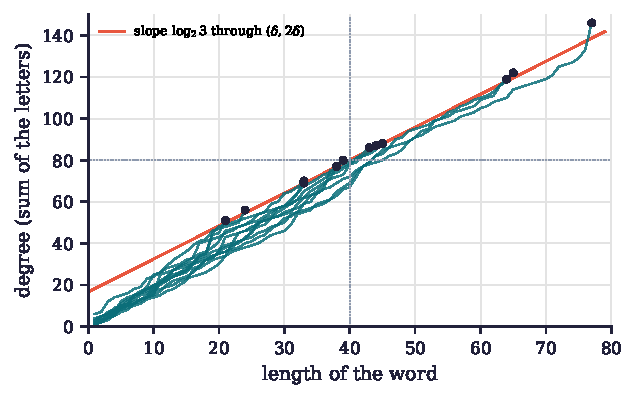
\includegraphics[width=\textwidth]{figures/ch9b_crossing.pdf}
\caption{First crossings at scale $\delta=40$ for twelve random words (of fourteen drawn, two do not cross within $80$ letters). Each path is the degree of a random word against its length; the dot marks the first crossing, after length $2\delta/5=16$, of the line of slope $\lt$ through $(\delta,2\delta)$, on which the weight $3^d2^{-\deg w}$ equals $(3/4)^\delta$, and the word is cut there.}
\label{fig:ch9b:crossing}
\end{figure}

A word in $\mathrm{FC}(\delta,R)$ of length $|w|$ and degree $\deg w=|w|\lt+(2-\lt)\delta+o$, where $0\le o\le R$ is its overshoot, has
\[
  \wt(w)=3^{|w|}2^{-\deg w}=(3/4)^{\delta}\,2^{-o},
\]
independent of its length. So by \eqref{eq:ch9b:offset} each block multiplies the source by about $(4/3)^{\delta}2^{o}$, whatever the length of the block, and the weights of all words built from the same sequence of blocks lie within a factor $2^{R_1+\cdots+R_j}$ of one another.

The \emph{weighted density}
\[
  Z_j(t)=\sum_{w\in L_j}\wt(w)\,\rho_{\lfloor\delta_j/4\rfloor}(s_w),
\]
where $L_j$ is the family of words of generation $j$ valid at $t$ and $s_w$ the source of $w$, weighs each word by the residue density of its source, that is, by the total weight of the words that can continue it (\cref{prop:ch9b:density}). Before the restriction to words valid at $t$, the words of generation $j$ form the family $\bar L_j$ of concatenations of $j$ first crossing blocks, where for $j\ge5$ the first five blocks must pass Lau's five block selector, a set of bounds on their rounded offsets that keeps the offset of every selected word between $85/256$ and $637/256$; its mass is $\mathrm{mass}(\bar L_j)=\sum_{w\in\bar L_j}2^{-\deg w}$. Fine scale mixing (\cref{prop:ch9b:mixing}) gives the propagation bound, which is summable.

\begin{proposition}[{Propagation, Lau~\cite[Proposition~6.1]{lau2026}, making explicit Mazur~\cite[Proposition~3.1]{mazur2026time}}]\label{prop:ch9b:propagation}
For every $j\ge6\times10^6$,
\[
  |Z_{j+1}(t)-Z_j(t)|\le Fj^{5/2}\,1.01^{-j},\qquad F=\tfrac92(C+1),\quad\log_2F<87534.2,
\]
with $C$ the constant of \eqref{eq:ch9b:mixing}.
\end{proposition}

From $j_0=6103914$ on, the remaining errors are small: they sum to less than $\frac54\cdot2^{-24}$, so that $Z_j(t)>2^{-25}$ for every $j\ge j_0$ wherever $Z_{j_0}(t)>2^{-23}$. At $j_0$ the function $Z_{j_0}$ is periodic modulo $3^{2^{87639}}$ and averages $\frac32\,\mathrm{mass}(\bar L_{j_0})>2^{-23}$ over the units, so some residue class $y_0$ has $Z_{j_0}>2^{-23}$. A seed $t_1=(2^at-1)/3$ in the class $y_0$ starts the construction from a general target, a terminal block places the sources in $[X,32X)$, and a census inequality, using the bound $8m^\alpha$ for the bounded part of the density, turns a terminal weighted density of at least $2^{-26}$ into $\beta_X(t)\ge2^{-160071}t^{-1.34}$; this is about where the exponent $160071$ comes from, since $2^{-26}/(8m^\alpha)\approx2^{-160068}$ at $m=2^{80000}$. Two small facts make the seed available: part (1) below is Lau's lemma on candidate residues, and part (2), with the use of two candidates, is from his Section~7.

\begin{lemma}[{Candidate seeds, after Lau~\cite{lau2026}}]\label{lem:ch9b:seed}
Let $3\nmid t$ and let $a_\circ\in\{38,39\}$ have $2^{a_\circ}t\equiv1\pmod3$. (1) For every $q\ge1$ and $i_0\ge0$, the integers $(4^{i}\,2^{a_\circ}t-1)/3$ for $i_0\le i<i_0+3^{q}$ meet every residue class modulo $3^{q}$ exactly once. (2) If two odd integers $y\ne y'$ satisfy $S(y)=S(y')$, at most one of them lies on a cycle of $S$.
\end{lemma}

\begin{proof}
For (1), the numbers are integers since $4^i2^{a_\circ}t\equiv2^{a_\circ}t\equiv1\pmod3$. The difference of the integers at $i<i'$ is $4^{i}2^{a_\circ}t\,(4^{e}-1)/3$ with $e=i'-i$, and $\nu_3(4^{e}-1)=1+\nu_3(e)$, which one checks by induction on $\nu_3(e)$. If $3\nmid e$, then $4^e-1=3(1+4+\cdots+4^{e-1})$ and the second factor is $\equiv e\not\equiv0\pmod3$, since $4\equiv1\pmod3$. If $3\mid e$, put $x=4^{e/3}\equiv1\pmod3$; then $4^e-1=(x-1)(x^2+x+1)$ and $x^2+x+1\equiv3\pmod9$, so $\nu_3(4^e-1)=\nu_3(4^{e/3}-1)+1$. Since $3\nmid t$ and $e<3^q$, the difference has $3$ adic order $\nu_3(e)<q$, and the $3^{q}$ integers are pairwise incongruent. For (2), if $S^{(j)}(y)=y$ and $S^{(j')}(y')=y'$ then with $r=jj'$ both are fixed by $S^{(r)}$, and $y=S^{(r-1)}(S(y))=S^{(r-1)}(S(y'))=y'$.
\end{proof}

Lau takes two candidates $t_1=(2^at-1)/3$ with $a=a_\circ+2i$ in the class $y_0$ modulo $3^{d_0}$, one with $i<3^{d_0}$ and one with $3^{d_0}\le i<2\cdot3^{d_0}$; by (1) each range contains exactly one. Both map to the odd part of $t$ in one step of $S$, so by (2) at least one is off every cycle, and \cref{lem:ch9b:distinct} applies to it. This is the only place cycles enter the argument, and they enter only to be avoided.

Read through \cref{chap:stochastic}, the propagation bound says that $Z_j$ is conserved from one generation to the next up to summable errors, as the expectation of a martingale is conserved under optional stopping. This is where the backward argument meets the martingale methods of this book.

\section{The two step constants are one constant}\label{sec:ch9b:constants}

\begin{proposition}[Steps of $T_0$ and steps of $S$]\label{prop:ch9b:steps}
Let the orbit of $n$ under $T_0$ reach $1$, let $m_1,\ldots,m_{A(n)}$ be its odd values before $1$, and let $H(n)=\sigma_0(n)-A(n)$ be its number of halvings. Then $2^{H(n)}=n\,3^{A(n)}\prod_i\bigl(1+\frac1{3m_i}\bigr)$, so that
\begin{equation}\label{eq:ch9b:steps}
  \sigma_0(n)=(1+\lt)A(n)+\log_2n+\varepsilon(n),\qquad \varepsilon(n)=\sum_{i=1}^{A(n)}\log_2\Bigl(1+\frac1{3m_i}\Bigr)\ge0 .
\end{equation}
\end{proposition}

\begin{proof}
An odd step multiplies the current value $m$ by $3(1+\frac1{3m})$ and a halving divides it by $2$, and the product of all these factors takes $n$ to $1$. Take logarithms to base $2$ and add $A(n)$.
\end{proof}

A bound $A(n)\le c\log n$ therefore gives $\sigma_0(n)\le\bigl((1+\lt)c+1/\log2\bigr)\log n+\varepsilon(n)$, and
\[
  (1+\lt)\cdot3.4881+\frac1{\log2}=10.4593<10.46 .
\]
This is how the two constants of \cref{thm:ch9b:lau} are tied: the bound for steps of $T_0$ follows from the bound for steps of $S$ in this way, with $\varepsilon$ absorbed by replacing $\log3$ with $\log(3+\frac1{4096})$, which is Mazur's condition $c_{\mathrm{acc}}\bigl(\log2+\log(3+\frac1{4096})\bigr)+1\le\frac{523}{50}\log2$ for a constant $c_{\mathrm{acc}}$ of accelerated steps. At the level of the model the same identity reads
\[
  \frac{1+\lt}{\log(4/3)}+\frac1{\log2}=\frac3{\log(4/3)},
\]
which is equivalent to $\log\frac43=(2-\lt)\log2$. So $3/\log(4/3)\approx10.428$ and $1/\log(4/3)\approx3.476$ are the drift constants of the stride model, $\log\frac34$ per stride and $\frac13\log\frac34$ per step of $T_0$, read backwards: a stride is on average $1+\E K=3$ steps of $T_0$. For the accelerated map, whose steps each contain one halving, the same count gives the slope $2/\log(4/3)=\gamma_0\approx6.952$ of \cref{chap:stochastic}.

\section{Step counts below \texorpdfstring{$3\cdot10^6$}{3 million}}\label{sec:ch9b:steps}

\Cref{tab:ch9b:steps} and \cref{fig:ch9b:steps} give $\sigma_0(n)$ and $A(n)$ for every $n$ with $10^4\le n<3\cdot10^6$, even and odd. Two points stand out. The share of $n$ meeting both of Lau's bounds is about $0.54$, against the proven $D_A^{-1}$: the tower is an artefact of the proof, not of the phenomenon. And the two bounds hold for exactly the same $n$ in every range. By \eqref{eq:ch9b:steps} the conditions $\sigma_0(n)\le10.46\log n$ and $A(n)\le3.4881\log n$ differ only when $A(n)$ lies between $3.4881\log n$ and $3.48837\log n-0.387\,\varepsilon(n)$, an interval of length $|0.0003\log n-0.387\,\varepsilon(n)|$, and no $n$ in the table has $A(n)$ there.

\begin{table}[t]
\centering\footnotesize
\caption{Steps of $T_0$ and of $S$ for $10^4\le n<3\cdot10^6$: the mean and standard deviation of $\sigma_0(n)/\log n$, the renewal prediction $16.42/\sqrt{\log n}$ for the standard deviation at the midpoint of the range, the mean of $A(n)/\log n$, and the share of $n$ meeting both of Lau's bounds $\sigma_0(n)\le\lfloor10.46\log n\rfloor$ and $A(n)\le\lfloor3.4881\log n\rfloor$. In every range the two bounds hold for exactly the same $n$.}
\label{tab:ch9b:steps}
\begin{tabular}{@{}lccccc@{}}
\toprule
range of $n$ & mean $\sigma_0/\log n$ & sd & predicted sd & mean $A/\log n$ & share \\
\midrule
$[10^4,10^5)$ & $10.219$ & $4.73$ & $4.97$ & $3.387$ & $0.552$ \\
$[10^5,10^6)$ & $10.258$ & $4.31$ & $4.52$ & $3.404$ & $0.541$ \\
$[10^6,3\cdot10^6)$ & $10.264$ & $4.11$ & $4.31$ & $3.407$ & $0.539$ \\
\bottomrule
\end{tabular}
\end{table}

\begin{figure}[t]
\centering
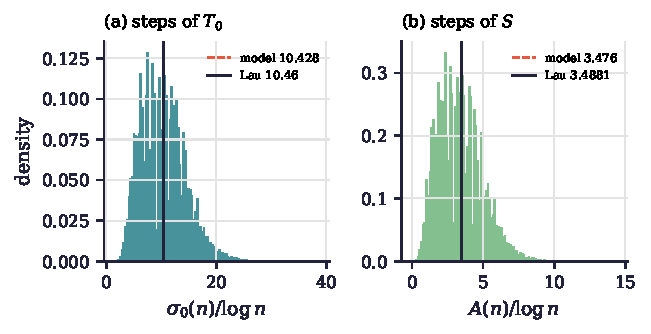
\includegraphics[width=\textwidth]{figures/ch9b_steps.pdf}
\caption{Steps to reach $1$ for $10^6\le n<3\cdot10^6$. (a) Histogram of $\sigma_0(n)/\log n$, with the model constant $3/\log(4/3)\approx10.428$ (dashed) and Lau's $10.46$ (solid). (b) Histogram of $A(n)/\log n$, with $1/\log(4/3)\approx3.476$ and Lau's $3.4881$. The comb comes from dividing integers by $\log n$ over a narrow range of $n$.}
\label{fig:ch9b:steps}
\end{figure}

The spread is the renewal\index{renewal} central limit theorem of \cref{sec:ch3:clt}. In the stride model a stride changes $\log x$ by $\log3-K\log2$, up to the plus one of \cref{rem:ch3:plusone}, with mean $\log\frac34$ and variance $2(\log2)^2$, since $K$ has variance $2$. The number of strides $A(n)$ is the first passage time below $0$ from $\log n$, and \eqref{eq:ch3:clt} gives
\[
  \frac{A(n)}{\log n}\approx\frac1{\log(4/3)}+\frac{\sqrt2\log2}{(\log\frac43)^{3/2}}\,\frac{Z}{\sqrt{\log n}},\qquad \frac{\sqrt2\log2}{(\log\frac43)^{3/2}}=6.353,
\]
with $Z$ standard normal. By \eqref{eq:ch9b:steps}, $\sigma_0$ inherits the factor $1+\lt$, so the standard deviation of $\sigma_0(n)/\log n$ is about $16.42/\sqrt{\log n}$. For the accelerated map the same identity reads $\sigma_\infty(n)=\lt A(n)+\log_2n+\varepsilon(n)$, and it turns the variance of the stride model into $(\lt)^2\cdot6.353^2\log n\approx101.4\log n$, the variance that \cref{sec:ch3:clt} computes from the coin model of $T$: the two models agree, as they must. The prediction in \cref{tab:ch9b:steps} is about five percent high throughout, consistent with the orbits being slightly less dispersed than the independent model at these sizes.

The consequence for Lau's constant is stark. The margin above the limiting mean is $10.46-3/\log(4/3)=0.0318$, so the share of $n$ meeting the bound $10.46\log n$ is roughly $\Phi\bigl(0.0318\sqrt{\log n}/16.42\bigr)$, which differs from one half by less than one percent for every $n$ below $10^{12}$, where a census is possible. The excess over one half in \cref{tab:ch9b:steps} comes from finite size: at these sizes the mean of $\sigma_0(n)/\log n$ is about $10.26$, below its limit, and the law is skewed to the right. Ninety percent coverage needs $\log n\approx4.4\times10^5$, an $n$ of about $190\,000$ digits, and ninety nine percent about $626\,000$ digits. Shaik's threshold is therefore the natural endpoint: for $c<3/\log(4/3)$ the same calculation sends the share to zero, which is the heuristic content of Problem~\ref{prob:ch11:b3}.

\section{The offset law in exact arithmetic}\label{sec:ch9b:offsets}

The mixing input can be tested directly. The offset of a word satisfies $\off(a\,v)=2^{-a}\bigl(1+3\off(v)\bigr)$, and $3\off(v)$ modulo $3^d$ depends only on $\off(v)$ modulo $3^{d-1}$, so $\pi_d$ is obtained from $\pi_{d-1}$ exactly:
\[
  \pi_d(z)=\sum_{a\ge1}2^{-a}\sum_{y:\ 2^{-a}(1+3y)\equiv z}\pi_{d-1}(y) .
\]
We evaluate this with the letters truncated at $a\le60$ and renormalized, which moves $\pi_d$ by at most $d\,2^{-60}$ in total variation, for $d\le18$, where $3^{18}\approx3.9\times10^8$, with a full Fourier transform at every level. \Cref{tab:ch9b:offsets} and \cref{fig:ch9b:fourier} report the largest Fourier coefficient at frequencies prime to $3$, the frequency attaining it, and the mean distances of $\rho_d$ from the lifts of $\rho_{d-1}$ and $\rho_{\lceil d/2\rceil}$. Four things stand out.

\begin{table}[t]
\centering\footnotesize
\setlength{\tabcolsep}{4pt}
\caption{The exact $3$ adic offset law. For each level $d$: the largest Fourier coefficient of $\pi_d$ at frequencies prime to $3$, the frequency in $[1,3^d/2]$ attaining it, that coefficient times $d^2$, the mean distance $3^{-d}\sum_y|\rho_d(y)-\rho_m(y\bmod3^m)|$ for $m=d-1$ and for $m=\lceil d/2\rceil$, and the largest value of $\rho_d$.}
\label{tab:ch9b:offsets}
\begin{tabular}{@{}rcccccc@{}}
\toprule
$d$ & $\max_{3\nmid\xi}|\widehat\pi_d(\xi)|$ & worst $\xi$ & $d^2\max|\widehat\pi_d|$ & $m=d-1$ & $m=\lceil d/2\rceil$ & $\max\rho_d$ \\
\midrule
$4$ & $0.1770$ & $2^{4}$ & $2.83$ & $0.343$ & $0.535$ & $7.27$ \\
$8$ & $0.0609$ & $2^{9}$ & $3.90$ & $0.213$ & $0.459$ & $37.3$ \\
$10$ & $0.0383$ & $2^{12}$ & $3.83$ & $0.178$ & $0.436$ & $84.2$ \\
$12$ & $0.0265$ & $2^{14}$ & $3.81$ & $0.151$ & $0.414$ & $189.6$ \\
$14$ & $0.0191$ & $2^{17}$ & $3.75$ & $0.130$ & $0.393$ & $426.8$ \\
$16$ & $0.0144$ & $2^{20}$ & $3.69$ & $0.112$ & $0.373$ & $960.3$ \\
$17$ & $0.0125$ & $2^{21}$ & $3.62$ & $0.104$ & $0.345$ & $1440.6$ \\
$18$ & $0.0112$ & $2^{23}$ & $3.62$ & $0.097$ & $0.354$ & $2160.9$ \\
\bottomrule
\end{tabular}
\end{table}

\begin{figure}[t]
\centering
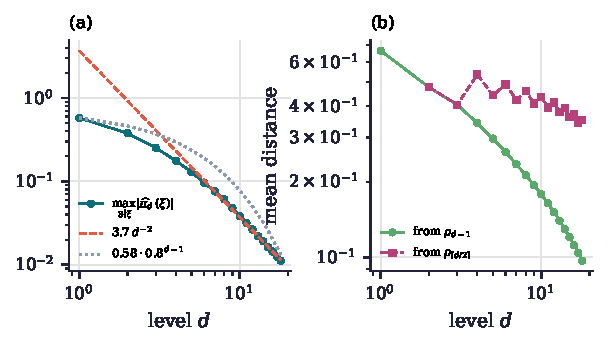
\includegraphics[width=\textwidth]{figures/ch9b_fourier.pdf}
\caption{The exact offset law, levels $1$ to $18$. (a) The largest Fourier coefficient of $\pi_d$ at frequencies prime to $3$, against $3.7\,d^{-2}$ (dashed) and the geometric curve $0.58\cdot0.8^{d-1}$ (dotted). (b) The mean distance of $\rho_d$ from the lift of $\rho_{d-1}$ and from the lift of $\rho_{\lceil d/2\rceil}$.}
\label{fig:ch9b:fourier}
\end{figure}

\begin{enumerate}
\item The decay is not geometric over this range. The ratio of consecutive maxima climbs from $0.65$, between levels $1$ and $2$, to $0.89$, between levels $17$ and $18$, while $d^2\max_\xi|\widehat\pi_d(\xi)|$ is nearly flat, drifting from $3.9$ at $d=8$ to $3.6$ at $d=18$ (it stays between $3.62$ and $3.90$ for $7\le d\le18$). Locally the decay looks like a power of $d$ near $2$, slowly steepening. This is consistent with Tao's theorem, which gives decay faster than any power asymptotically, but it says that the preasymptotic regime is long.
\item The worst frequency is a power of $2$. Since $2$ generates the units modulo $3^d$, every frequency prime to $3$ is a power of $2$ modulo $3^d$; the point is that the maximizing frequency, taken in $[1,3^d/2]$, is a power of $2$ as an integer, at every level $d\le18$, with every frequency prime to $3$ scanned: $2^k$ with $d\le k\le1.28\,d$ for $2\le d\le18$ ($k/d=1.278$ at $d=18$, where $k=23$). \Cref{tab:ch9b:profile} shows the profile of $|\widehat\pi_d(2^k)|$ over $k$ for $d=14$ to $18$: a smooth bump in $k$, about six values of $k$ wide at half its height, whose peak moves right by one or two per level. Multiplication by $2$ is the symmetry generated by the letters, and a plausible reason is that a frequency $2^k$ sees the first letter through the small integer $2^{k-a_1}$, where the cancellation is weakest. Any sharp bound will have to treat this orbit of frequencies separately, much as Lau's black triangles do.
\item The residue density is far from bounded: $\max\rho_d$ grows by a factor $\frac32$ per level (between $1.50004$ and $1.50014$ at levels $15$ to $18$), like the weight $(3/2)^d$ of the word of $d$ ones (\cref{ex:ch9b:ones}). This is why the census uses a bounded part of the density in place of $\rho_m$ itself.
\item Mixing across levels is slow. The distance from the lift of $\rho_{d-1}$ falls only like $d^{-0.84}$ over $4\le d\le18$ ($d^{-0.97}$ over $8\le d\le18$), and the distance from the lift of $\rho_{\lceil d/2\rceil}$ is still $0.35$ at $d=18$. A bound of the form $Cm^{-3/2}$ with $m=\lceil d/2\rceil$, as in \eqref{eq:ch9b:mixing}, holds at these levels only with $C\ge9.5$, and the constant needed rises steadily ($8.45$ at $d=16$, $9.31$ at $d=17$, $9.55$ at $d=18$). Lau's bound starts at $m\ge2^{80000}$, and these levels say nothing about whether a constant as large as his is needed there.
\end{enumerate}

\begin{table}[t]
\centering\footnotesize
\setlength{\tabcolsep}{3pt}
\caption{The profile of the worst frequency: $|\widehat\pi_d(2^k)|$ for $d=14$ to $18$ and $k=16$ to $27$, blank where $2^k>3^d$. The largest entry of each row is underlined; it equals the maximum over all frequencies prime to $3$ at that level.}
\label{tab:ch9b:profile}
\begin{tabular}{@{}rcccccccccccc@{}}
\toprule
$d$ & \multicolumn{12}{c}{$k$} \\
\cmidrule(l){2-13}
 & $16$ & $17$ & $18$ & $19$ & $20$ & $21$ & $22$ & $23$ & $24$ & $25$ & $26$ & $27$ \\
\midrule
$14$ & $0.0178$ & $\underline{0.0191}$ & $0.0177$ & $0.0136$ & $0.0083$ & $0.0043$ & $0.0020$ &  &  &  &  &  \\
$15$ & $0.0111$ & $0.0143$ & $\underline{0.0163}$ & $0.0162$ & $0.0137$ & $0.0095$ & $0.0054$ & $0.0023$ &  &  &  &  \\
$16$ & $0.0059$ & $0.0085$ & $0.0113$ & $0.0136$ & $\underline{0.0144}$ & $0.0132$ & $0.0103$ & $0.0065$ & $0.0032$ & $0.0014$ &  &  \\
$17$ & $0.0029$ & $0.0044$ & $0.0064$ & $0.0089$ & $0.0111$ & $\underline{0.0125}$ & $0.0124$ & $0.0106$ & $0.0075$ & $0.0043$ & $0.0020$ &  \\
$18$ & $0.0014$ & $0.0021$ & $0.0032$ & $0.0048$ & $0.0068$ & $0.0090$ & $0.0106$ & $\underline{0.0112}$ & $0.0104$ & $0.0082$ & $0.0054$ & $0.0028$ \\
\bottomrule
\end{tabular}
\end{table}

The question is therefore not one of spectral gaps, since the model chain modulo $3^a$ reaches its stationary law $\pi_a$ exactly in $a$ strides (\cref{lem:ch9:mixing}), but one about the fine structure of $\pi_d$ itself: the true exponent of its worst Fourier coefficient, in the preasymptotic range and asymptotically (Problem~\ref{prob:ch11:b2}).

\section{The backward view and the rest of the book}\label{sec:ch9b:book}

\Cref{tab:ch9b:book} lines up the backward proof against the themes and open problems of this book.

\begin{table}[t]
\centering\footnotesize
\caption{Where the backward proof of Mazur and Lau touches this book.}
\label{tab:ch9b:book}
\begin{tabular}{@{}>{\raggedright}p{0.24\textwidth}>{\raggedright}p{0.38\textwidth}>{\raggedright\arraybackslash}p{0.30\textwidth}@{}}
\toprule
In this book & In the backward proof & Relation \\
\midrule
Drift $\log\frac34$ and the stride model (\cref{chap:stochastic}) & Geometric letters of mean $2$; $\log\wt$ is a random walk with drift $\log\frac34$; Lau's Lemma~11.9 is a submartingale stopped at a first passage & The same model, run backwards: weights of predecessors rather than sizes of iterates \\
Large deviations (\cref{chap:parity,chap:stochastic}) & Cram\'er and Chernoff tails for the degree, Hoeffding bounds, explicit moment generating functions & A shared toolkit; the bounds in the proof are explicit \\
Continued fractions of $\lt$ (\cref{chap:cycles}) & Lines of slope $\lt$; $\lceil n\lt\rceil$, the bit length of $3^n$; the convergent $19/12$ through $3^{12}>2^{19}$; the brackets $79/50<\lt<317/200$ & The book explains why such rationals appear; the proof uses them \\
O1 and the divergence half (Problem~\ref{prob:ch11:o1}) & Nothing about divergent orbits; but convergence on a set of density one would exclude them (\cref{cor:ch9b:densityone}) & None in method; a density statement now reaches O1 \\
O2, trajectory mixing (Problem~\ref{prob:ch11:o2}) & Tao's fine scale mixing for one iterate, with an explicit polynomial rate & The closest contact: O2 asks for the same transfer along a whole orbit \\
O3, O3$'$, certificates & Not used & None \\
O4, the third cumulant (Problem~\ref{prob:ch11:o4}) & Not used & The renewal computation of \cref{sec:ch9b:steps} is its second order analogue \\
O5, uniform integrability (Problem~\ref{prob:ch11:o5}) & Summable propagation errors for $Z_j$; bounded stopping times & An analogous role for a different object \\
Cycles (\cref{sec:ch11:cycles}) & Avoided by choosing seeds; no cycle bounds & None in method; once density one is known, cycles are irrelevant \\
Parity autocorrelations (\cref{sec:ch3:autocorr}) & Independent letters in the model, paid for by mixing & The proof measures how far true residues are from independent ones \\
Optimization (Part~II) & Not used & None \\
Machine checked statements (\cref{sec:ch8:lean}) & Lean formalizations of the main theorems & An explicit theorem about the Collatz map, checked by machine \\
\bottomrule
\end{tabular}
\end{table}

The overlap is in the probability model and in the arithmetic of $\lt$, not in the argument. The book works forwards: it treats $\log T^{(k)}(n)$ as a supermartingale with drift $\ds$, majorizes it, accelerates it, and asks for equidistribution and integrability to close the gap. Mazur and Lau work backwards: they count predecessors, weigh them by $3^d2^{-\deg w}$, and need only that the offsets mix modulo powers of $3$. These are dual views of one random walk, and until now this book had only the forward one.

The backward results sharpen three open problems, listed in \cref{chap:open} as B1 to B3: a bounded form of Tao's theorem (Problem~\ref{prob:ch11:b1}), which by \cref{prop:ch9b:bounded} would settle the conjecture; the true decay rate of the Fourier coefficients of $\pi_d$ (Problem~\ref{prob:ch11:b2}), of which \cref{sec:ch9b:offsets} is a first measurement; and the sharpness of Shaik's constant $3/\log(4/3)$ (Problem~\ref{prob:ch11:b3}).

What the results do not do should be said plainly. They prove nothing about the orbit of any particular integer. They say nothing about cycles beyond avoiding them. The proportion they guarantee, $D_A^{-1}$, is unimaginably small, while the share of integers meeting the step bounds is about one half at every size we can compute and, by the renewal calculation, tends to one. And they are recent and unrefereed: Lau's mathematics was produced by AxiomProver, and Mazur's first manuscript underwent automated reviews, not human peer review~\cite{mazur2026pred}. The Lean formalizations are the strongest reason to trust the statements. Mazur cautions that formal verification does not replace a check that the formal statements match the informal ones~\cite{mazur2026time}; for Lau's theorem we have made that check on the statements, as \cref{sec:ch9b:theorems} records, but we have not run the proofs.

\section*{Notes}

This chapter grew out of a reading note on Lau's preprint written for this book in October 2026. The examples, the backward tree table and figure, the section on the $2$ adic and $3$ adic models, the seed lemma and several of the exercises come from the first author's draft of this chapter. Lau's preprint is hexagon:2610.00249v1 on the Hexagon preprint server, with its source; Mazur's manuscripts are on proofatlas.ai, with their Lean sources; Shaik's preprint is on Zenodo, with its source. The statements of \cref{thm:ch9b:lau}, \cref{cor:ch9b:densityone} and the history in \cref{sec:ch9b:theorems} were compared with those texts, and Lau's Lean statements were read in the challenge file of his repository at its commit of 15 October 2026. Mazur's manuscript of July 2026 on natural density is cited from the description in~\cite{mazur2026time}. Lau cites Tao by the numbering of the corrected arXiv version of July 2026; in the version of February 2022, Propositions~1.14 and~1.17 have the same numbers.

\begin{sloppypar}The computations of \cref{sec:ch9b:words,sec:ch9b:steps,sec:ch9b:offsets} are by the scripts \texttt{ch9b\_tree.py}, \texttt{ch9b\_steps.py}, \texttt{ch9b\_offset\_law.py} and \texttt{ch9b\_figures.py} (\cref{app:code}). The offset law to level $18$, with a full transform at every level, took about ten minutes and under $30$ gigabytes on a cluster node; at level $19$ ($3^{19}\approx1.2\times10^9$) the law fits in memory but the library's transform failed, so levels $19$ and $20$ remain to be computed. The mean distances from the lift of $\rho_{d-1}$ in \cref{tab:ch9b:offsets} are twice the total variation distances of \cref{sec:ch9:tao}, and at levels $2$ to $7$ they reproduce the values $0.238$, $0.203$, $0.171$, $0.149$, $0.131$, $0.117$ given there.\end{sloppypar}

\section*{Exercises}

\begin{exercise}\label{ex:ch9b:ones}
Prove the composition rules of \cref{prop:ch9b:offset}, and use them to show that the word of $d$ ones has offset $(3/2)^d-1$, and that every word of length $d$ has $0<\off(w)\le(3/2)^d-1$, with equality only for the word of $d$ ones. Deduce that the word of $d$ ones is valid exactly at the odd $n\equiv-1\pmod{3^d}$, where it contributes $(3/2)^d$ to $\rho_d$.
\end{exercise}

\begin{exercise}\label{ex:ch9b:targetone}
Show that each odd $s>1$ is the source of exactly one word $w_s$ valid at $1$ whose orbit $s,S(s),\ldots,1$ meets $1$ only at its last term, that the other words valid at $1$ with source $s$ are the $(2,\ldots,2,w_s)$ with one or more initial letters $2$, which carry three times the weight of $w_s$ in all, and that $1-\off(w_s)=2^{-\varepsilon(s)}$ with $\varepsilon$ as in \cref{prop:ch9b:steps}. Deduce that $\beta_X(1)=\sum_s2^{-\varepsilon(s)}/s<\sum_s1/s$, the sums over the odd $s$ in $[X,32X)$.
\end{exercise}

\begin{exercise}\label{ex:ch9b:units}
Show that $2$ generates the units modulo $3^d$, and deduce that every unit modulo $3^d$ is the offset of a word of length $d$, so that $\rho_d>0$ exactly on the units. Interpret both halves of this statement in the inverse tree.
\end{exercise}

\begin{exercise}\label{ex:ch9b:rhothree}
Compute $\rho_3$ on the eighteen units of $\Z/27\Z$ and check that it averages to $\tfrac32$ and that the lift of $\rho_2$ differs from it by about $0.41$ on average, as in \cref{fig:ch9b:fourier}(b).
\end{exercise}

\begin{exercise}\label{ex:ch9b:conditional}
Prove that the forward letters of a random odd $2$ adic integer are independent geometric variables (\cref{thm:terras}, \cref{prop:geom}), and that the backward letters of a random word, conditioned on validity at a fixed target $n$, are not independent, although they stay independent if the target is uniform modulo $3^d$. Which conditional law do they have at a fixed target?
\end{exercise}

\begin{exercise}\label{ex:ch9b:densities}
Show that for every $A\subseteq\N$ the lower natural density is at most the lower logarithmic density, which is at most the upper logarithmic density, which is at most the upper natural density. (Write $\sum_{n\le x,\,n\in A}1/n$ by partial summation in terms of $A(y)=\#\{n\le y:n\in A\}$.) Deduce the form of \cref{cor:ch9b:densityone} in \cref{prop:ch9b:bounded}.
\end{exercise}

\begin{exercise}\label{ex:ch9b:three}
Show that if $3\mid t$, the integers whose orbit under $T_0$ reaches $t$ are exactly the $2^kt$ with $k\ge0$.
\end{exercise}

\begin{exercise}
Prove the identity $\frac{1+\lt}{\log(4/3)}+\frac1{\log2}=\frac3{\log(4/3)}$, interpret each side as an expected number of steps per unit of $\log n$, and check that $(1+\lt)\cdot3.4881+1/\log2<10.46$. Which constant for steps of $S$ corresponds in the same way to Shaik's threshold $3/\log(4/3)$?
\end{exercise}

\begin{exercise}
In the stride model, compute the mean and the variance of $\log3-K\log2$, and derive the constant $\sqrt2\log2/(\log\frac43)^{3/2}\approx6.353$ of \cref{sec:ch9b:steps} from \eqref{eq:ch3:clt}. Show that the identity $\sigma_\infty(n)=\lt A(n)+\log_2n+\varepsilon(n)$ for the steps of $T$ turns it into the variance $101.4\log x_0$ of \cref{sec:ch3:clt}.
\end{exercise}

\begin{exercise}\label{ex:ch9b:coverage}
Using the renewal variance $2(\log2)^2/(\log\frac43)^3$ of \cref{sec:ch9b:steps} and ignoring the finite size bias of the mean, estimate the size of $n$ at which the bound $\sigma_0(n)\le c\log n$ holds for ninety five percent of integers, for $c=10.46$, $10.5$ and $11$.
\end{exercise}
